
%
% Chapter 4
%

\chapter{Object reconstruction and event generation}
\label{chap:event_sim}
\section{Introduction}
\label{intro}
This chapter is divided into two parts. In the first part, the procedure for the generation of simulated events is described. This is done in several distinct stages with the output of one stage serving as an input for the next. A suite of software packages, developed mostly by the particle and nuclear physics communities, is used to achieve this. This part concludes by detailing the simulated datasets used in the analyses described in this thesis. In the second part of this chapter, the reconstruction of physics objects is described in detail. It starts with a description of the particle-flow algorithm which is kind of a global event reconstruction scheme for the entire event. This is followed by descriptions of track , muon and electron reconstructions. Reconstruction of jets is described next followed by description of composite objects used in the analysis such as collinear mass and transverse mass. Brief desciptions of tau lepton reconstruction and b-tagging of jets is also included.


\section{Event Simulation}
A $pp$ collision at the LHC, like any hadronic collision, is more complex than the hard interaction of two participating partons. The proton being a composite object, the colliding partons from the hard interaction are accompanied by other quarks and gluons that interact and rearrange themseleves into colorless objects. A $pp$ collision thus consists of: the Hard Scattering which represents the part of the collision where two partons in the initial state interact by exchanging a high transverse momentum, and the Underlying Event that represent the interaction of the everything else in the collision except the partons in hard scattering. In addition to the implementing the above, i.e. physics of a $pp$ collision  that produces a bunch of final state particles, the event simulation also has to include interactions of these particles with the CMS detector. Monte Carlo methods, that use generation of random numbers to simulate sampling from a given probability distribution , are used to model the above event simulations~\cite{mc_evtsim}.

\subsection{Monte Carlo method}

Monte Carlo (MC) methods (named after a famous casino in the city state of Monaco) are a broad class of computational algorithms that rely on repeated random sampling to obtain numerical results~\cite{mcwiki}. In particle physics, these methods play a key role in generation of events and are used primary for : generation of samples from specified probabilty distributions, and the calculation of integrals. Programs which implement the above method, called MC event generators, use generation of random numbers to make decisions about physics processes. These can range from selection of processes are generated in the collision, to which decay channel a particle decays in, to making decisions on how the particle interacts with detector material. Usually, each such decision is the result of a draw from a distribution which depends only on the current state the process is in, and not on previous states. The MC generator is provided as input the distributions that represent the physics of the generated particles, their production, their decay modes and their couplings. A MC generator starts by using a pseudo-random number generator that usually outputs a random number between 0 and 1 with. Although, true random number generation can only be done by physical processess, modern pseudo-random number generators are known to generate numbers with a high degree of randommness. Starting from this distribution, the MC event generator uses one of the various methods such as the inverse-transform method, or the rejection sampling method to convert this uniform distribution into a desired probablity distribution, $p(x)$. It is then possible to generate random numbers according to this distribution to simulate physical processes. 


\subsection{CMS simulation pipeline}

The MC simulation of events in CMS consists of the following sequential steps. The first step is simulation of the Hard Scattering.As mentioned earlier, this represents the primary hard interaction in a collision where two partons in the initial state interact by exchanging high transverse momentum resulting in a final state with two or more partons. The parton density function (pdf) which parametrizes the distributions of the partons inside each hadron are used to model the momenta of incoming partons. It represents the probability of finding a parton of a certain flavour at a certain longitudinal momentum fraction, when the hadron, that contains it, is probed at a certain scale. The PDF are extracted from fits to the data, mainly from ep collisions, and various PDF sets are available for each parton flavour. Commonly used pdf sets include ones provided by the  CTEQ, HERA (H1 and ZEUS) and NNPDF collaborations. The LHAPDF library provides a unified C++ interface to all major PDF sets. The matrix element formulation is used to model the hard scattering process to leading order in perturbative QCD, or to higher orders depending on the generator. The next step is simulation of the parton shower. The hadronization and radiation of quarks and gluons in the initial and final states cannot be feasibly encapsulated in the matrix element computation. Parton shower describes these missing parts. The matrix element calculations are combined with the parton shower by one of the different matching schemes which ensure that there is no double counting of terms present in both the matrix element and the partion shower expansion. The matching schemes that are most often used are MLM~\cite{mlm}, CKKW~\cite{ckkw} and FxFx~\cite{Frederix:2012ps}. The simulation of the Underlying Event comes next. Underlying event includes everything in the collision that is not associated with the primary hard scattering process. They consist mostly of soft QCD interactions, and implemented using the MC event generators and interfaced with the matrix element simulation. The hadronization of the quarks and gluons is simulated next and it conisists of recombination of individual partons into colorless hadrons. Lastly the decay of short-lived particles is simulated.

An important part of the event generation chain is the simulation of pileup. The protons circulate inside the LHC not as a continuous beam but in discrete closely packed bunches. This leads to more than one proton-proton collision per bunch crossing, i.e. pileup both in-time and out-of-time (see chapter~\ref{chap:exper_setup}). Event generators add  pile-up events to the hard scattering samples by randomly simulating soft inelastic collisions and overlapping them. The distribution of the number of pileup interactions in data is hard to predict. MC event generators usually produce events for a scenario with a higher number of pileup vertices, and with a flat disctribution of number of vertices . This is afterwards reweighted to match the observed distribution of pileup interactions in data.

Several MC generators have been developed. Some of these can produce all components of the above simulation pipeline while some calculate only the matrix element and need to be interfaced with other generators for the simulation of remaining parts. Pythia~\cite{Sjostrand:pythia8} and Herwig~\cite{herwig} can produce the entire chain while Powheg~\cite{Nason:2004rx,Frixione:2007vw, Alioli:2010xd, Alioli:2010xa, Alioli:2008tz, Bagnaschi:2011tu}, aMC@NLO~\cite{Alwall:2014} and Madgraph~\cite{Alwall:2011uj} produce up to matrix element stage. Powheg and aMC@NLO can perform next-to-leading order calculations. 

Finally, the Geant4 (GEometry ANd Tracking)~\cite{GEANT4} package is used to simulate the interaction of physical particles after the collision, produced by pipeline described  above, with a sophisticated and complex simulation of the detector itself. This simulated detector response is used as input for the same physics reconstruction algorithms (desribed in the next section), that are used to reconstruct the data, thus enabling a direct comparison of the two. If differences are observed in the behavior of these reconstruction algorithms for MC events in comparsion to observed data, the MC events are tuned to the behavior observed in data. 


\section{MC samples used for the analyses}
\label{samples_mc}

The {ggH} and VBF Higgs boson samples are generated with POWHEG 2.0 while an extension of POWHEG 2.0~\cite{Luisoni:2013kna} is used for the $\PW\PH$ and $\PZ\PH$ simulated samples. For the \Hmue analysis, only the gluon fusion (ggH) production mode has been considered. Samples are generated for a range of H masses from 200 to 900 GeV.

The $\zjets$ and $\wjets$ processes are simulated using the \aMCATNLO generator at leading order (LO) with the MLM jet matching and merging scheme. The same generator is also used for diboson production which is simulated at  next-to-LO (NLO) with the FxFx jet matching and merging scheme. POWHEG 2.0 and 1.0 are used for top quark-antiquark ($\ttb$) and single top quark production, respectively. The POWHEG and MADGRAPH generators are interfaced with PYTHIA 8 for parton showering, fragmentation, and decays. 

As mentioned earlier in this chapter, additional pileup interactions are also a part of the MC generation pipeline. All simulated samples are reweighted to the pileup distribution observed in data. An event weight is applied based on the number of simulated pileup events and the instantaneous luminosity per bunch-crossing, averaged over the run period. Several other scale factors  are used to reweight the events in order to get the MC simulation to match the data closely. These include scale factors based on trigger, lepton identification, lepton isolaton and b-jet tagging efficiencies.

\section{Physics Object Reconstruction}
\label{p_ob_recon}
This section begins with the description of the particle-flow algorithm followed by reconstruction of tracks and vertices, electrons, muons, jets and other physics objects.  
\subsection{Particle Flow}
\label{p_flow}
\subsection{Track and primary vertex reconstruction}
\label{track_recon}

Tracks of charged particles, that traverse the CMS tracker (described in section~\ref{tracker}), are reconstructed~\cite{track_reconstruction} using hits from the pixel and strip detectors in the tracker. Hits are reconstructed by clustering signals above specified thesholds in the pixel and strip channels, and then estimating the cluster positions and uncertainties in a local orthogonal system plane of each sensor. During track reconstruction, a translation is made between the local coordinate system of these hits to the global coordinate system of the tracks. The software used to reconstruct tracks by CMS is called the Combinatorial Track Finder (CTF) and is adaptation of the Kalman filter~\cite{kalman_filter}. Tracks are reconstructed using a iterative procedure with the basic idea being, that tracks that are easiest to find (e.g., high \pt tracks, and produced near the interaction region) are searched in the initial iterations with subsequesnt iterations looking for more difficult sets of tracks (e.g., low \pt tracks , or tracks produced far from the interaction region). Hits unambiguously assigned to the track in the previous iterations are removed for the subsequent ones, thus reducing the combinatorial complexity. Each iteration can be divided into four sequential steps.

The first step is seed generation which provides initial track candidates that define the starting trajectory parameters and associated uncertainties of potential tracks. Charged particles follow a helical paths in the quasi-uniform magnetic field of the tracking requiring a total of five parameters to determine the trajectory. These five parameters are extracted using two or three hits in the inner region of the tracker. The seeds are constructed in the inner part (and then tracks constructed outwards, and not in the opposite manner) because the high granularity of pixel detectors (in contrast to outer strip layers)  ensure low fraction of channels that are hit. Also, particles like pions and electrons interact inelastically with tracker material or lose energy due to bremsstrahlung radiation as they traverse through the tracker to its outer regions making the idea of construcing seeds in the inner region a better choice.

The second step in track generation is track finding which is closely based on the Kalman filter. It extrapolates the seed trajectories along the expected path of a charged particle, beginning with an estimate of the track parameters provided by the trajectory seeds generated in the last step. It then uses the location and uncertainty of detected hits, and estimations of effects such as Coulomb scattering, at successive detector layers, to build track candidates, updating the parameters at each layer. First, using the parameters of the track candidate, evaluated at the current layer, an analytical extrapolation is done that determines which adjacent layers of the detector the trajectory can intersect. This takes into account the current uncertainty in that trajectory just like a Kalman filter. Secondly, a search is perfomed for silicon modules in these layers that are compatible with the extrapolated trajectory. All compatible modules in each layer are then grouped into mutually exclusive groups, such that no two modules in each group overlap. The collection of all hits from from one such module group forms a group of hits. Finally, new track candidates are formed by adding exactly one of the compatible hits from each group, to each original track candidate. The modules in a given group are mutually exclusive and a contribution of more than one hit from each group is not expected. The trajectory parameters of the new candidates are then updated by combining the information from the added hits with the extrapolated trajectory of the original track candidates. Fig~\ref{fig:trackrecon} illustrates the reconstruction efficiency of tracks in case of isolated muons.

The third step in track generation track fitting. In this step the collection of hits from the last step are refitted using a Kalman filter and smoother, to provide a best possible estimate of parameters for each track trajectory. The procedure described above, in conditions as challenging as the LHC, can yields several fake tracks that are not associated with any charged particle passing through the tracker. The fourth and final step applies several quality requirements to set of reconstructed tracks and substantially reduces the fake contribution. The requirements are based on criteria such as the minimum number of layer the track has hits in, how compatible its origin is with a primary vertex, how good a fit they yield etc.

\begin{figure*}
\begin{center}
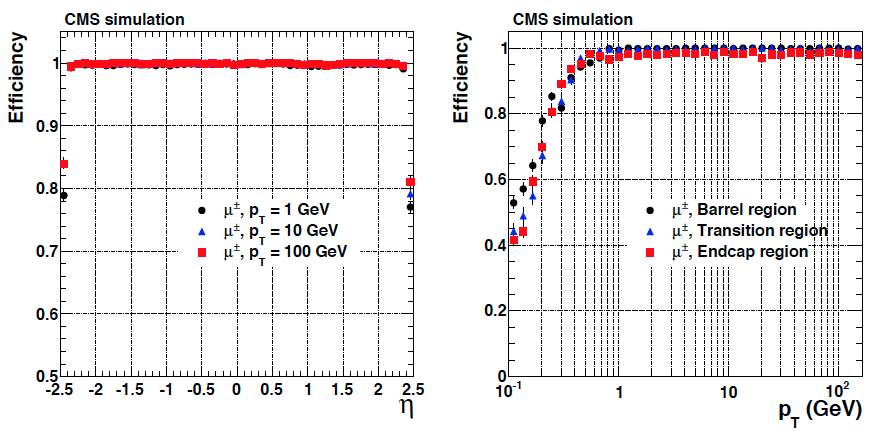
\includegraphics[width=0.9\textwidth,keepaspectratio]{plots_and_figures/chapter4/trackrecon.png}
\caption{Track reconstruction efficencies for single isolated muons as a function of $\eta$ and \pt~\cite{track_reconstruction}.}
\label{fig:trackrecon}
\end{center}
\end{figure*}


Proton-proton interaction vertices are reconstructed by selecting tracks that are produced promptly in the primary interaction region. The selected tracks are then clustered on the basis of their z-coordinatesat their point of closest approach to the centre of the beam spot, which represents a 3-D profile of the region where the LHC beams collide inside the CMS detector. The exact positions of the vertices are then obtained from these clustered candidates, by using a fitting procedure, called the adaptive vertex fitter~\cite{vertex_fitting}. The vertex which has the largest sum of squared transverse momenta of tracks originating from it is considered the primary interaction vertex. 


\subsection{Muon Reconstruction}
\label{mu_recon}
Hits in the muon system (described in section ~\ref{muon_system}) and tracks (muons being charged particles leave tracks in the tracker) from the tracker are used to reconstruct muons~\cite{muon_recon2018}. When muons traverse a muon subdetector (such as RPC, CSC or DT) in the muon system, they ionize the gas in the chambers. The electrical signals produced on the wires and strips as a consequence of the ionization are read out by electronics systems that associate these ``hits'' with well-defined locations in the detector. Various algorithms depending on the subdetector technology are used to reconstruct these hits. Reconstruction of muon tracks using these hits first proceeds independently of track reconstruction in the tracker. These tracks, called \textit{standalone-muon tracks}, are built using these reconstructed hits from the muon system using a Kalman filter. Muon tracks are also built inside-out by propagating tracker tracks (described in previous section) with transverse momentum above 0.5 GeV to the muon system and matching them to (straight-line) segments of hits in DT or CSC. If a match is found, the tracker track qualifies as a \textit{tracker muon track}. Muon tracks are also  built outside-in  by matching standalone-muon tracks with tracker tracks, and combining information from both using a Kalman filter fit. These are called \textit{global muon tracks}. While the global muon reconstruction is especially efficient for muons leaving hits in several muon stations. The \textit{tracker muon} reconstruction is more efficient for low \pt muon candidates but it can also cause fake muon tracks due to hadronic particles which \textit{punch-through} to the innermost muon stations. The \textit{global muon} reconstruction has  high efficiency for muons penetrating through more than one muon station, and reduces the muon misidentification rate compared to tracker muons. Combining both \textit{tracker muon tracks} and \textit{global muon tracks}, the efficiency for reconstructing a muon is as high as 99\%. The particle-flow algorithm applies a set of requirements, based on various quality parameters from muon reconstruction as well as information from other sub-detectors, to  reconstructed candidates. The PF muon candidates used in the analyses described in this thesis were required to satisfy the following set of criterion to be identified as a muon:

\begin{itemize}
\item Must be a global muon or a tracker muon.
\item Must have at least one hit in the pixel subdetector of the tracker
\item $\chi^2$ of the compatibility between the position of the standalone and trackers tracks $<12$
\item Transverse impact parameter of the associated tracker track with respect to the primary vertex $d_{xy}< 2 mm$
\item Longitudinal distance of the (origin of )associated tracker track with respect to the primary vertex $d_z <5 mm$
\item constraints on muon segment matching compatibility between tracker and muon system dependent on if it is a global muon
\end{itemize}
The efficiency of the above selection for muon identification is illustrated using a plot from a study performed by the CMS Muon Physics Object group in Fig.~\ref{fig:muoneff}. As can be seen from the plots, there is a difference in the efficiencies in data and MC simulation. This is corrected using a set a of scaled factors applied as a function $\eta$ and \pt to adjust the efficiency in simulation to get it to match the efficiency in data.  

\begin{figure*}[!htpb]\centering
 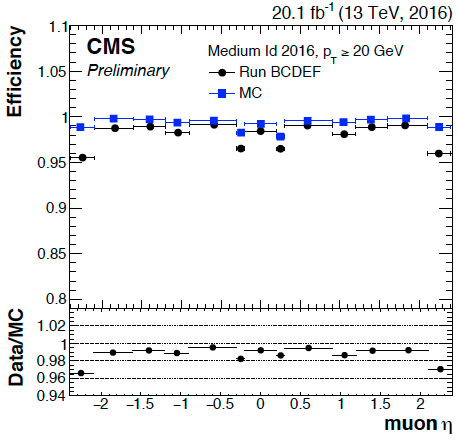
\includegraphics[width=0.47\textwidth]{plots_and_figures/chapter4/muoneffveta.png}
 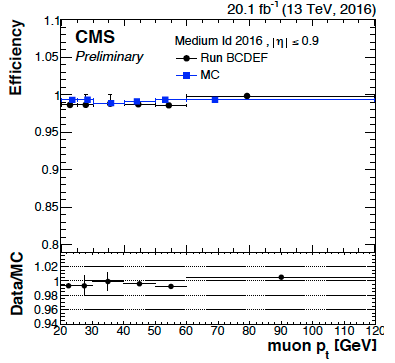
\includegraphics[width=0.49\textwidth]{plots_and_figures/chapter4/muoneffvpt1.png} \\
 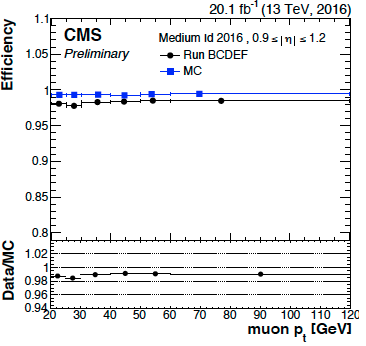
\includegraphics[width=0.49\textwidth]{plots_and_figures/chapter4/muoneffvpt2.png}
 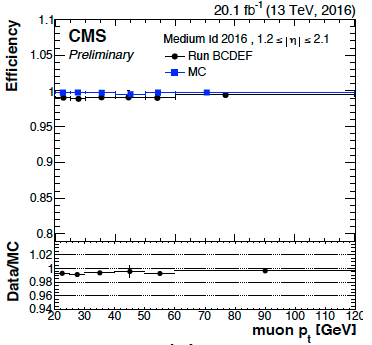
\includegraphics[width=0.49\textwidth]{plots_and_figures/chapter4/muoneffvpt3.png} 
\caption{Efficiency of muon identification as a function of $\eta$ and \pt, for data (black) and simulation (blue)}
 \label{fig:muoneff}
\end{figure*}  
  
The momentum of muons is measured by CMS using one among different possible ways involving the tracker and muon system~\cite{muon_recon2012} and then using the PF algorithm to refine this informmation that exploits information from the full event.








\subsection{Electron Reconstruction}
\label{e_recon}
Besides muons, electron form the other primary part of the final state of the decay we are searching for in this thesis. Electrons, in the CMS, are reconsrtucted using clusters of energy formed in the ECAl (described in section ~\ref{Ecal}) and associating them with tracks from the tracker. The reconstruction of electrons is made complicated by the fact that they can radiate a significant amount of energy before reaching the ECAL. This happens due to the radiation of bremsstrahlung photons caused by the ineraction of electrons with atoms as they pass through the tracker. This loss can range from 33\% to as high as 86\% depending on $\eta$ (as a consequence of the fact that the amount of detector material the electron has to cross is $eta$ dependent). In order to measure the an electron's energy,  clustering algorithms thus need to take into the energy from these bremsstrahlung photon showers together with the deposit made in the ECAL by the electron. The energy from these radiated photons spreads primarily in the $\phi$ owing to bend in electron trajectory in the magnetic field of CMS. The spread in the $\eta$ direction is relatively small. These facts are used by the clustering algorithms.

The algorithm used to cluster the electron energy deposit in the ECAL barrel is called the \textit{hybrid} algorithm. It exploits the above property of the electron shower shape, and uses the geometry of the ECAL to form clusters thare are narrow in $\eta$ direction but wide in $\phi$ direction. Starting with a (seed) crystal containing the largest amount of energy deposited in a considered region above a certain threshold (1 GeV), it adds 5x1 arrays of crystals in $\eta\times\phi$ around the seed crystals in both directions of $\phi$ if the energy contained in the arrays is above another predefined threshold (0.1 GeV). Contiguous arrays are merged into clusters, and finally a electron supercluster is formed from all such strip clusters which have at least one seed strip with energy above another predefined threshold (0.35 GeV). The position of the supercluster is computed as the energy-weighted mean of the cluster positions, whereas its energy is simply taken as the sum of the energy of all its constituent clusters. In the ECAL endcap a different clustering algorithm is used owing to different geometrical arrangement of the crystals. This algorithm called the \textit{5x5} algorithm starts similarly with a seed crystal with maximum energy in a local region, and satisfying the minimum energy requirement of 0.18 GeV. Clusters of 5x5 crystals are progressively grouped around the seed crystal, making a supercluster, if the total cluster energy exceeds 1 GeV and the are withing $\pm 0.7$  and $\pm 0.3$ respectively in $\eta$ and $\phi$ around the seed crystal. The positon and energy of the supercluster is calculates in the same manner as the barrel. The energy from the preshower is also added into the supercluster, using it's most energetic cluster and it's maximum distance in $\phi$ to other clusters and extrapolating it to the preshower plane to define the spread in the preshower. The thresholds used in the above algorithms were optimized using simulation and adjusted durting data taking periods.

The standard track reconstuction (section ~\ref{track_recon}) is not efficient for electrons. This is because the standard approach is compromised by the large radiative losses in the tracker leading to a poor estimation of track parameters. Therefore a dedicated tracking procedure is used for  electron candidated that used infromation not only from the tracker but also the ECAL. Just like the standard track reconstruction procedure the first step in electron track reconstruction is seeding. This is done in two ways and the results are then combined. In the first method, superclusters from ECAL are used. As mentioned earlier, owing to strong magnetic field, the bremsstrahlung photons emitted by the electrons deposit energy in the ECAL at $\η$ values similar to that of the electron, but at diffrent $\phi$ leading to a spread. The ECAL supercluster algorithms described above recover this energy. The position and  energy of these reconstructed superclusters along with the assumption that the electrons originated close to the center of the beam spot can be used to constrain the trajectory of the electron through the tracker. Hits in the first layers of the trackers compatible with these trajectories are deemed electron seeds. In the second method of seeding, the "opposite" is done. Tracks constructed by the regular tracking algorithm are extrapolated to the ECAL and matched with a supercluster. The seeds corresponding to such matching tracks are retained as electron seeds. The seed collections from these two methods are merged leading to a increase in overall efficiency of the seeding procedure. These seeds are then used to intiate electron track finding.








\subsection{Jet Reconstruction}
\label{jet_recon}
\subsection{MET, MT and Collinear Mass}
\label{col_mass}
\subsection{Tau Lepton and others}
\label{tau_recon}


\section{Datasets}
\label{datasets}

The data analysed in this search was gathered by the CMS detector in 2016 during proton-proton collisions at the LHC, corresponding to an integrated luminosity of $35.9 fb^{-1}$. This data corresponds to a center-of-mass energy of 13 TeV and a spacing of 25ns between bunch crossings in the LHC with an average of about 30 collisions per bunch crossing. The subset of samples used among all collected by CMS are the ones having at least one isolated muon having transverse energy over 24 GeV, as triggered by the CMS high level isolated muon trigger (HLT\_IsoMu24 in CMS parlance).




% % uncomment the following lines,
% if using chapter-wise bibliography
%
% \bibliographystyle{ndnatbib}
% \bibliography{example}

% % uncomment the following lines,
% if using chapter-wise bibliography
%
% \bibliographystyle{ndnatbib}
% \bibliography{example}
